\chapter{Neural Networks}
\begin{quotation}
\noindent ``\emph{The question of whether a computer can think is no more 
	interesting than the question of whether a submarine can swim.}''
\begin{flushright}\textbf{Edsger W. Dijkstra}\end{flushright}
\end{quotation}

\vspace*{0.5cm}

Throughout this paper, we will use the very powerful tool that a neural network
is for several different purposes. One could describe a neural network in 
three words: general function approximators. We can describe their input
and the output desired from that input -- inbetween, a very large amount of
nonlinear computations of which coefficients and parameters can be tuned to
make the network's output closer to what we want in a process called training, 
or learning. The name "neural network"
barely hides the analogy with how human neurons function -- and although there
are similarities to how humans learn, the analogy stays very much a conceptual
analogy, and artificial neural networks stay orders of magnitude less complex
than the billions and billions of interconnected neurons humans have developed. 

\section{Feedforward neural networks}
A neural network is a collection of interconnected \textit{neurons}. The
simplest and most widely used networks are feedforward neural networks. In this
setting, neurons are arranged into ordered layers of which the first one is
called the input layer, and the last one is called the output layer.\\

The input vector is composed of \textbf{features}; measures, properties. Say
for example that we wanted to build a neural network that classifies cats and
dogs; we could measure attributes such as the height of the animal, the length
of its hair, its general loyalty to its owners and the number of hours it 
spends sleeping per day.\\

For the output layer, we would have a two-neuron layer: one which corresponds
to "cat" and the other one to "dog". Once we have trained the network
(see Section~\ref{nn:training}), the neuron that has the highest value
after distilling the input values through the network would specify the
kind of animal the neural network thinks the measurements best fit to.\\

\begin{figure}[]
	\centering
	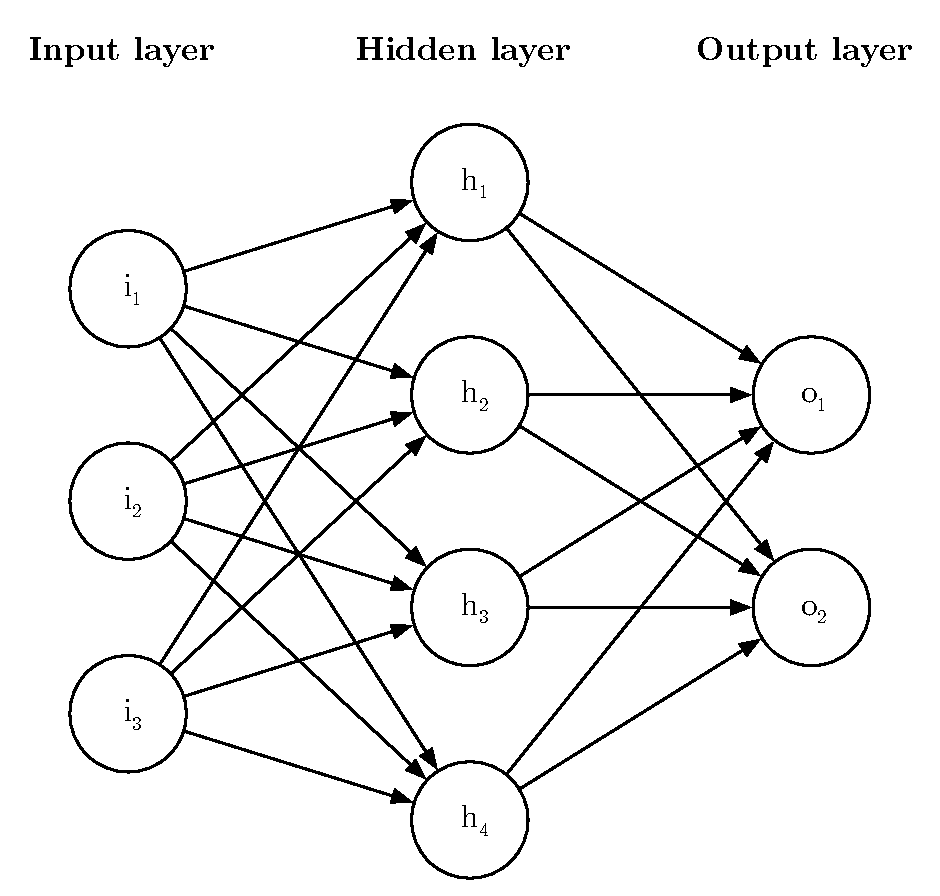
\includegraphics[width=0.6\linewidth]{fig/neural_network.eps}
	\caption{A neural network with one input layer composed of three neurons,
	one hidden layer of 4 neurons, and one output layer with 2 neurons.}
	\label{fig:neural_network}
\end{figure}


In a feedforward neural network, each neuron is connected to every neuron in 
the next layer.  To obtain an output from a given input,
the information will be passed from layer to layer in the following way : 
each neuron computes a weighted sum of the outputs of all neurons in the
previous layer then squashes this weighted sum in an activation function
\index{activation function}. 
Hence, the neuron $h_1$ in the network of Figure~\ref{fig:neural_network}
outputs:
$$ f(w_1i_1 + w_2i_2 + w_3i_3 + b) $$
where $w_1, w_2, w_3$ are the weights \index{weights} corresponding to the
connections between $i_1, i_2, i_3$ and $h_1$; and $b$ is a bias term. 
These weights are the learnable parameters of any neural network and will be 
tuned during training to improve the accuracy of the network. 
The activation function $f(\cdot)$ can be chosen arbitrarily, as long as it 
is differentiable (so that backpropagation can work, see \ref{nn:training})
but it is the same for all the neurons in the same layer. Some options are
the sigmoid function, the hyperbolic tangent function and sometimes a simple
linear function.\\

The reader might have noticed that using matrices is an efficient way of writing
and executing computations within a neural network. Indeed, one could write
the computation between the input layer and the first hidden layer as: 

$$ h = f(iW_{ih} + b_h) $$

\noindent where : 
\begin{itemize}
	\item $h$ is a $1\times n$ vector containing the values of the neurons 
		in the hidden layer
	\item $i$ is a $1\times m$ vector containing the values of the neurons
		in the input layer
	\item $W_{ih}$ is a $m\times n$ matrix containing the weights between
		the input and hidden layer
	\item $b_h$ is the $1\times n$ bias vector 
\end{itemize}

\subsection{Training}
\label{nn:training}
Every neural network is initialised randomly at first, meaning that we will
attribute a random value (that is sampled from a user-defined distribution)
to each weight in the network.\\

If we want to train a network to differentiate a cat from a dog based on a
given set of measurements, we will have to show it a large number of examples
of measurements and their associated ground truths \index{ground truth}
(whether the measurements actually correspond to a cat or a dog). This large
number of examples is called the \textbf{training set} \index{training set}.
Training is
then performed by alternating feedforward passes (distilling the input through
the network and obtaining the network output) and backpropagation, modifiying 
the weights of the connections between neurons (that will in turn modify 
the network output) until the network output matches the ground truth with 
a good enough accuracy.\\

The forward pass has been explained previously, but the backwards pass, also
called \textbf{backpropagation}, is slightly more complicated.\\

\subsubsection{Loss function}
The first thing we need to make our network better is a number which tells us
how far the network output is from the ground truth.
This is exactly what a \textbf{loss function} \index{loss function} does: 
it describes numerically the error between the target and the network output.
One example of a loss function is the mean square error (MSE) \index{MSE}:
$$ \mathcal{L} = (t-p)^2$$
where $t$ is the target, or the ground truth, and $p$ is the prediction. In
many cases, $t$ and $p$ are vectors, so we may sum or average the loss computed
over components.
In our cats and dogs example, let us consider that the ground truth for
"cat" corresponds to the output vector $[1, 0]$ and the ground truth for "dog"
corresponds to the output vector $[0, 1]$. If the network predicts $[0.3, 0.7]$
when it is given measurements of a cat, the loss function will equate to :
$$ \mathcal{L} = ([1, 0]-[0.3, 0.7])^2 = (1-0.3)^2 + (0-0.7)^2 = 0.98$$
whereas if it had predicted $[0.9, 0.1]$, the loss would have equated to:
$$ \mathcal{L} = ([1, 0]-[0.9, 0.1])^2 = (1-0.9)^2 + (0-0.1)^2 = 0.02$$

The experienced reader might already have concluded that since we want to
minimise the loss function, we are confronted to an optimisation problem.

\subsubsection{Backpropagation}
\index{backpropagation}
We will only summarise backpropagation in this section as explaining it in
full is out of the scope of this paper.
The problem at hand is indeed an optimisation problem with the following
parameters:
\begin{itemize}
	\item the objective function is the loss function
	\item the parameters are all the weights of the neural network
\end{itemize}
How can we link the parameters to the objective function? A key requirement
for activation functions and the loss function is that they have to be
\textbf{differentiable}. When this is the case, we can compute the gradient
of the loss function and backpropagate it through the network by using the
chain rule of derivation. The first question to ask is: how do the weights
of the last layer affect the loss function? We can get a glimpse of this
by looking at the partial derivatives of the loss function regarding those
weights:
$$\nabla\mathcal{L} = \left(
  \frac{\delta\mathcal{L}}{\delta w_1}, 
  \frac{\delta\mathcal{L}}{\delta w_2}, 
  \frac{\delta\mathcal{L}}{\delta w_3}, ...,
  \frac{\delta\mathcal{L}}{\delta w_k}\right) 
$$
for each weight in the network. Each weight will then be modified by adding
$$ \Delta w_i = - \alpha \frac{\delta\mathcal{L}}{\delta w_i}$$
where $\alpha$ is the learning rate.\\

Backpropagation uses the fact that activation functions are differentiable to
perform gradient descent. Indeed, the error signal is a surface in a space
of which the dimensionality is equal to the number of parameters in the
network. Gradient descent aims to find the global minimum of this error
surface.\\


\subsubsection{Summary}
To train a neural network, its weights have to be randomly initialised first,
then we show it many examples of the training set, containing measurements and
ground truths. For each of these examples, or samples:
\begin{enumerate}
	\item the feedforward pass computes the network output from the sample
		input data
	\item the network output is compared with the sample output and the
		error signal given by a loss function
		is backpropagated through the network, updating
		all the weights
\end{enumerate}


\section{Recurrent neural networks}
There is one limitation to feedforward neural networks which can be particulary
critical for some applications. Very often, having an output mapped to a 
single input is not enough. For example, in problems where samples are organised
in a timeline and dependent on each other, only seeing one input at a time
does not provide enough information. If one wants to predict the weather
temperature in the next hour, it would be useful to know more than only the
last ground truth value to identify a potential trend. One 
could input a fixed-size window of the previous time steps to the network,
but this approach limits the scope of available "memory" and could dramatically
increase the complexity of the model.\\

One solution to this problem is the use of recurrent neural networks.
A feedback loop such as the one shown in Figure~\ref{fig:rnn}a, also called
a recurrent connection, means that the layer at the receiving end of the
recurrent connection will receive as input not only the value of the previous
layer at time $t$, but also the value of the layer at the giving end of the 
recurrent connection at time $t-1$. This allows information to \textit{live}
throughout time steps.\\

A recurrent connection, however, poses evident issues for the backpropagation
algorithm since the depth of the neural network can become theoretically
infinite.  A common way of training and visualising recurrent neural networks 
is to unroll them for a given, finite amount of time steps (see 
Figure~\ref{fig:rnn}b).  The error signal can then be computed
for the output value at each time step, and backpropagated through all the
previous input values that affected its computing.\\

\begin{figure}[]
	\centering
	\subfloat[][A recurrent connection]{\qquad
		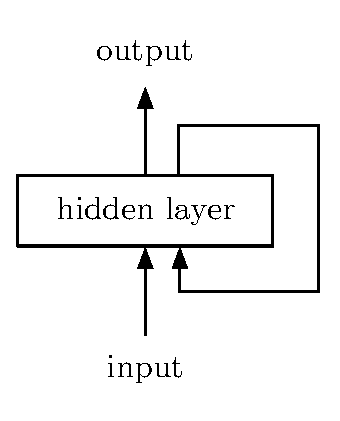
\includegraphics[width=0.1515\linewidth]{fig/recurrent_neural_network.eps}\qquad}
	\qquad
	\subfloat[][An unrolled recurrent neural network]{
		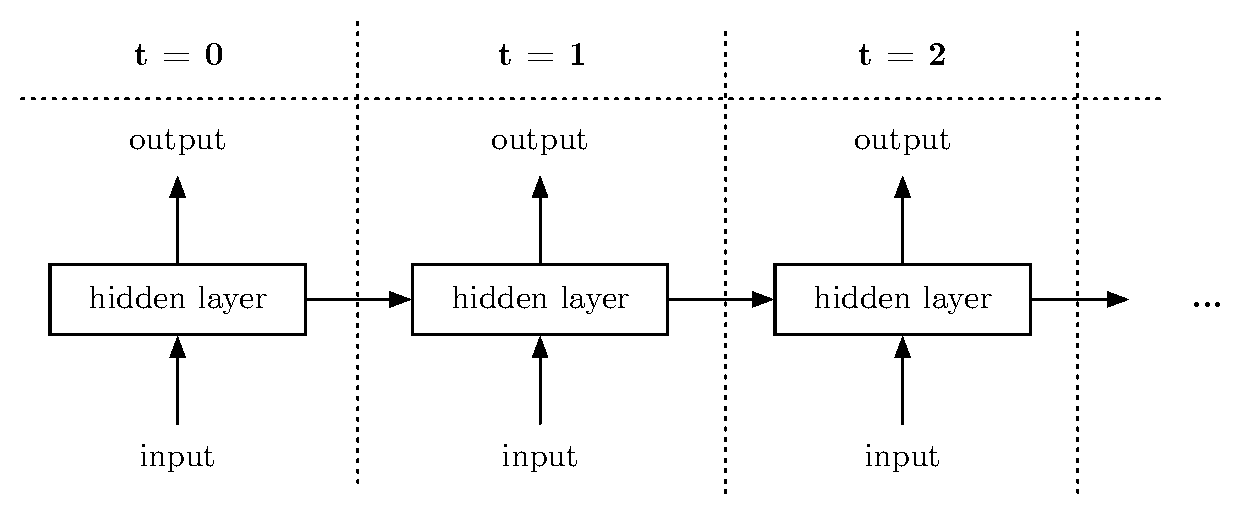
\includegraphics[width=0.6\linewidth]{fig/recurrent_neural_network_unrolled.eps}}
	\caption{Recurrent neural networks}
	\label{fig:rnn}
\end{figure}

\subsection{Long Short-Term Memory (LSTM)}
\todo{universal function approximators}


